% Options for packages loaded elsewhere
\PassOptionsToPackage{unicode}{hyperref}
\PassOptionsToPackage{hyphens}{url}
%
\documentclass[
  man]{apa6}
\usepackage{amsmath,amssymb}
\usepackage{lmodern}
\usepackage{iftex}
\ifPDFTeX
  \usepackage[T1]{fontenc}
  \usepackage[utf8]{inputenc}
  \usepackage{textcomp} % provide euro and other symbols
\else % if luatex or xetex
  \usepackage{unicode-math}
  \defaultfontfeatures{Scale=MatchLowercase}
  \defaultfontfeatures[\rmfamily]{Ligatures=TeX,Scale=1}
\fi
% Use upquote if available, for straight quotes in verbatim environments
\IfFileExists{upquote.sty}{\usepackage{upquote}}{}
\IfFileExists{microtype.sty}{% use microtype if available
  \usepackage[]{microtype}
  \UseMicrotypeSet[protrusion]{basicmath} % disable protrusion for tt fonts
}{}
\makeatletter
\@ifundefined{KOMAClassName}{% if non-KOMA class
  \IfFileExists{parskip.sty}{%
    \usepackage{parskip}
  }{% else
    \setlength{\parindent}{0pt}
    \setlength{\parskip}{6pt plus 2pt minus 1pt}}
}{% if KOMA class
  \KOMAoptions{parskip=half}}
\makeatother
\usepackage{xcolor}
\usepackage{graphicx}
\makeatletter
\def\maxwidth{\ifdim\Gin@nat@width>\linewidth\linewidth\else\Gin@nat@width\fi}
\def\maxheight{\ifdim\Gin@nat@height>\textheight\textheight\else\Gin@nat@height\fi}
\makeatother
% Scale images if necessary, so that they will not overflow the page
% margins by default, and it is still possible to overwrite the defaults
% using explicit options in \includegraphics[width, height, ...]{}
\setkeys{Gin}{width=\maxwidth,height=\maxheight,keepaspectratio}
% Set default figure placement to htbp
\makeatletter
\def\fps@figure{htbp}
\makeatother
\setlength{\emergencystretch}{3em} % prevent overfull lines
\providecommand{\tightlist}{%
  \setlength{\itemsep}{0pt}\setlength{\parskip}{0pt}}
\setcounter{secnumdepth}{-\maxdimen} % remove section numbering
% Make \paragraph and \subparagraph free-standing
\ifx\paragraph\undefined\else
  \let\oldparagraph\paragraph
  \renewcommand{\paragraph}[1]{\oldparagraph{#1}\mbox{}}
\fi
\ifx\subparagraph\undefined\else
  \let\oldsubparagraph\subparagraph
  \renewcommand{\subparagraph}[1]{\oldsubparagraph{#1}\mbox{}}
\fi
\ifLuaTeX
\usepackage[bidi=basic]{babel}
\else
\usepackage[bidi=default]{babel}
\fi
\babelprovide[main,import]{english}
% get rid of language-specific shorthands (see #6817):
\let\LanguageShortHands\languageshorthands
\def\languageshorthands#1{}
% Manuscript styling
\usepackage{upgreek}
\captionsetup{font=singlespacing,justification=justified}

% Table formatting
\usepackage{longtable}
\usepackage{lscape}
% \usepackage[counterclockwise]{rotating}   % Landscape page setup for large tables
\usepackage{multirow}		% Table styling
\usepackage{tabularx}		% Control Column width
\usepackage[flushleft]{threeparttable}	% Allows for three part tables with a specified notes section
\usepackage{threeparttablex}            % Lets threeparttable work with longtable

% Create new environments so endfloat can handle them
% \newenvironment{ltable}
%   {\begin{landscape}\centering\begin{threeparttable}}
%   {\end{threeparttable}\end{landscape}}
\newenvironment{lltable}{\begin{landscape}\centering\begin{ThreePartTable}}{\end{ThreePartTable}\end{landscape}}

% Enables adjusting longtable caption width to table width
% Solution found at http://golatex.de/longtable-mit-caption-so-breit-wie-die-tabelle-t15767.html
\makeatletter
\newcommand\LastLTentrywidth{1em}
\newlength\longtablewidth
\setlength{\longtablewidth}{1in}
\newcommand{\getlongtablewidth}{\begingroup \ifcsname LT@\roman{LT@tables}\endcsname \global\longtablewidth=0pt \renewcommand{\LT@entry}[2]{\global\advance\longtablewidth by ##2\relax\gdef\LastLTentrywidth{##2}}\@nameuse{LT@\roman{LT@tables}} \fi \endgroup}

% \setlength{\parindent}{0.5in}
% \setlength{\parskip}{0pt plus 0pt minus 0pt}

% Overwrite redefinition of paragraph and subparagraph by the default LaTeX template
% See https://github.com/crsh/papaja/issues/292
\makeatletter
\renewcommand{\paragraph}{\@startsection{paragraph}{4}{\parindent}%
  {0\baselineskip \@plus 0.2ex \@minus 0.2ex}%
  {-1em}%
  {\normalfont\normalsize\bfseries\itshape\typesectitle}}

\renewcommand{\subparagraph}[1]{\@startsection{subparagraph}{5}{1em}%
  {0\baselineskip \@plus 0.2ex \@minus 0.2ex}%
  {-\z@\relax}%
  {\normalfont\normalsize\itshape\hspace{\parindent}{#1}\textit{\addperi}}{\relax}}
\makeatother

% \usepackage{etoolbox}
\makeatletter
\patchcmd{\HyOrg@maketitle}
  {\section{\normalfont\normalsize\abstractname}}
  {\section*{\normalfont\normalsize\abstractname}}
  {}{\typeout{Failed to patch abstract.}}
\patchcmd{\HyOrg@maketitle}
  {\section{\protect\normalfont{\@title}}}
  {\section*{\protect\normalfont{\@title}}}
  {}{\typeout{Failed to patch title.}}
\makeatother

\usepackage{xpatch}
\makeatletter
\xapptocmd\appendix
  {\xapptocmd\section
    {\addcontentsline{toc}{section}{\appendixname\ifoneappendix\else~\theappendix\fi\\: #1}}
    {}{\InnerPatchFailed}%
  }
{}{\PatchFailed}
\keywords{emotions, social cognition, perception, intergroup dynamics, open data, open materials, preregistered}
\DeclareDelayedFloatFlavor{ThreePartTable}{table}
\DeclareDelayedFloatFlavor{lltable}{table}
\DeclareDelayedFloatFlavor*{longtable}{table}
\makeatletter
\renewcommand{\efloat@iwrite}[1]{\immediate\expandafter\protected@write\csname efloat@post#1\endcsname{}}
\makeatother
\usepackage{lineno}

\linenumbers
\usepackage{csquotes}
\ifLuaTeX
  \usepackage{selnolig}  % disable illegal ligatures
\fi
\IfFileExists{bookmark.sty}{\usepackage{bookmark}}{\usepackage{hyperref}}
\IfFileExists{xurl.sty}{\usepackage{xurl}}{} % add URL line breaks if available
\urlstyle{same} % disable monospaced font for URLs
\hypersetup{
  pdftitle={Replication of Corrigendum: The Crowd-Emotion-Amplification Effect},
  pdfauthor={Liu Jiachen1, Yang Qingren1, \& Zhang Yilin1},
  pdflang={en-EN},
  pdfkeywords={emotions, social cognition, perception, intergroup dynamics, open data, open materials, preregistered},
  hidelinks,
  pdfcreator={LaTeX via pandoc}}

\title{Replication of Corrigendum: The Crowd-Emotion-Amplification Effect}
\author{Liu Jiachen\textsuperscript{1}, Yang Qingren\textsuperscript{1}, \& Zhang Yilin\textsuperscript{1}}
\date{}


\shorttitle{SHORT TITLE}

\authornote{

Each member of our group actively participated in every step of the replication process, but there was still a focus on division of labor. We had the following responsibilities: Liu Jiachen was primarily responsible for code verification, creating plots, and proofreading the manuscript; Yang Qingren primarily handled the Chinese manuscript and statistical verification; Zhang Yilin was primarily responsible for the English manuscript, presentation, and PowerPoint production.

}

\affiliation{\vspace{0.5cm}\textsuperscript{1} Nanjing Normal University}

\abstract{%
We replicated the first study of the article ``The Crowd-Emotion-Amplification Effect'' written by Amit Goldenberg, published in the journal ``Psychological Science'' in March 2021. This article investigates how people judge the emotions of a group of individuals by rapidly scanning their facial expressions. The researchers proposed that when people observe a group, they tend to focus on faces displaying strong emotions, leading to a phenomenon known as the crowd-emotion amplification effect, where the estimated average emotional response of the group is more extreme than the actual average.In the first study (N = 50), the researchers documented the crowd-emotion amplification effect. In the second study (N = 50), even with increased exposure time, the effect was successfully replicated. In the third study (N = 50), the researchers used eye-tracking technology to demonstrate that attention bias towards emotional faces drives the amplification effect. Through replicating this study, we gained a better understanding of the crowd-emotion amplification effect.
}



\begin{document}
\maketitle

\hypertarget{introduction}{%
\section{Introduction}\label{introduction}}

Imaging yourself making a speech in front a group of people, you quickly scan the audience, how can you make split-second judgements about the emotions of the crowd. This article proposes that perceivers preferentially attend to faces exhibiting strong emotions, as highly emotional faces are more salient than neutral faces (Pessoa et al., 2002), which in turn generates a crowd-emotional-amplification effect---estimating a crowd's average emotional response as more extreme than it actually is.
One explanation is that people preferentially attend to faces conveying strong emotions over faces with neutral expressions (Eimer \& Holmes, 2007; Pessoa et al., 2002). Thus, when a person infers a crowd's emotion, attentional bias toward more emotional faces should contribute to an amplification in the average emotion estimate.
When generating rapid evaluation of others' emotions, the capacity for visual representation is finite (Alvarez, 2011; Whitney \& Yamanshi Leib, 2018), ensemble coding compensates for this limitation by allowing perceivers to form compressed, summary representations of visual information (Whitney et al., 2014). While how these summaries are computed is still under debate. Whether people encode all items in a set or only a subset, it is plausible they preferentially attend to the most salient items in a set (Kanaya et al., 2018; Sweeny et al., 2013). Kanaya and colleagues (2018) explored this hypothesis, their experiments provided evidence of amplification in the estimation of multiple objects, however, it is thus unclear whether a similar effect of amplification would be evident with faces.
By replicating this study, we can further deepen our understanding of the crowd-emotion amplification effect. In the first study (N = 50), researchers documented the presence of the crowd-emotion amplification effect. In the second study (N = 50), even with increased exposure time, the effect was replicated. In the third study (N = 50), researchers employed eye-tracking technology to demonstrate that attentional bias toward emotional faces drives the generation of the emotion amplification effect. The results of these replicated studies enable us to gain a more comprehensive understanding of the characteristics and underlying mechanisms of the crowd-emotion amplification effect.
The significance of conducting replicated studies lies in several aspects. Firstly, replication allows us to validate and confirm the findings of the original study, ensuring the reliability and robustness of the observed effects. It helps establish the generalizability of the phenomenon under investigation and strengthens the overall body of knowledge in the field.

Secondly, replication provides an opportunity to examine the consistency and stability of the effects over different samples, settings, or conditions. By replicating the study with different participants or manipulating certain variables, we can explore the boundary conditions of the phenomenon and gain a deeper understanding of its underlying mechanisms.

Furthermore, replication allows for the identification of potential limitations or factors that may influence the observed effects. If the results of the replication study align with those of the original study, it enhances the confidence in the validity of the findings. On the other hand, if the results differ, it prompts further investigation into the factors contributing to the discrepancy and encourages critical evaluation and refinement of the original research.

Ultimately, the significance of replication lies in its contribution to the cumulative nature of scientific knowledge. It fosters transparency, rigor, and intellectual progress by encouraging researchers to build upon existing findings, challenge assumptions, and refine theories. Through replication, we can gain a more comprehensive and reliable understanding of the phenomenon under study, and its implications can extend to various fields, applications, and practical contexts.
Through an in-depth exploration of the crowd-emotion amplification effect, we can develop a more accurate understanding of the dynamic changes in emotions within a group and apply it in practical contexts. The significance of this research lies in providing valuable insights into how individuals make judgments about emotions when observing a crowd, while also reminding us of important considerations in social interaction and emotional cognition.

\hypertarget{research-hypothesis}{%
\section{Research hypothesis}\label{research-hypothesis}}

Based on the above research background, the study proposed three hypotheses.
Hypothesis 1 : Participants would show a crowd-emotion-amplification effect, estimating a crowd's average emotion as more intense than it actually is.
Hypothesis 2 : The amplification effect would be stronger as the number of faces within an array increased (following Kanaya et al., 2018).
Hypothesis 3 : Amplification would be more robust for negative emotions than for positive emotions.

\hypertarget{methods}{%
\section{Methods}\label{methods}}

\hypertarget{participants}{%
\subsection{Participants}\label{participants}}

After conducting a power analysis that suggested that a sample size of 50 participants completing 150 trials would provide power of 97\% to support the first hypothesis, they recruited 50 participants (23 men, 27 women; age: M = 19.52 years, SD = 1.69), each of whom completed 150 trials.

\hypertarget{procedure}{%
\subsection{Procedure}\label{procedure}}

In each trial, participants first saw an array containing 1 to 12 faces (Fig. 1). These faces expressed different intensities of emotion from either neutral-to-angry or neutral-to-happy continua (Fig. 2). The group-average intensity, the valence of the faces, and the set size were all chosen randomly on each trial. They did not mix the happy and angry faces in the same set for two reasons. First, doing so could undermine their ability to detect an amplification effect. Second, the most-happy and most-angry faces were not equal in intensity, thus making the average between the two different from zero.
They concatenated 50 modifications of a face from neutral to extremely angry and from neutral to extremely happy, effectively creating a visual rendering of 50-points anger or happiness scales. (Fig. 2). On every trial, an array containing between 1 and 12 faces was presented to participants. Faces could appear in any of 12 fixed locations on the screen.
The group's mean emotional intensity was randomly set to be between 10 and 40 (on the basis of a 50-point scale of angry or happy faces, 1 being neutral and 50 being very angry or very happy). They limited the range of the group means in order to allow distributions of intensity that were as close to uniform as possible within the 50-point scale. The sets were engineered so that the standard deviation of a 12-face array was always 10, from which they randomly chose a subset of 1 to 12 faces.
To prevent residual visual processing, they immediately followed each face in the array with a mask at the same location. After viewing the face array and the mask, participants were asked to evaluate the average emotion expressed in the array. They presented a single face bearing a neutral expression on the screen after the array was masked, so participants could make their evaluations.
After completing the main task, participants filled out a short survey that included an abbreviated version of the Social Interaction Anxiety Scale, the Need to Belong Scale, and demographic questions including age, gender, race, and education level.
Figure 2 A sample of three faces from the neutral-to-angry scale (top) and from the neutral-to-happy scale (bottom) that were used in the studies.
Results
To measure amplification in estimation of the face sets, they conducted a mix-model analysis of repeated measures, comparing the actual mean emotion expressed in each set with participant estimated mean emotion. The results show that the estimated mean crowd emotion was 1.87 points higher (scale from 1 to 50) than the actual mean crowd emotion, b = 2.87, 95\% confidence interval (CI) = {[}2.53, 3.21{]}, SE = 0.17, t(14533) = 16.8, p \textless{} .001, R2 = .05, which support the crowd-emotion-amplification hypothesis (Hypothesis 1).
They used a single mode to test whether an increase in the number of faces (Hypothesis 2) or the type of emotions expressed by the faces (Hypothesis 3) influenced the crowd-emotion-amplification effect. Results were in line with the second and the third hypothesis. Number of faces significantly predicted an increase in amplification, b = 0.42, 95\% confidence interval (CI) = {[}0.21, 0.64{]}, SE = 0.03, t(7233) = 3.86, p \textless{} .001, R2 = .08 (Fig 3). For hypothesis 3, amplification was stronger for crowds expressing negative emotions than crowds expressing positive emotions, b = 0.24, 95\% confidence interval (CI) = {[}0.02, 0.45{]}, SE = 0.11, t(7253) = 2.18, p = .02, R2 = .08. The interaction between number of faces and the valence expressed by the faces was not significant, b = 0.08, 95\% confidence interval (CI) = {[}-0.13, 0.30{]}, SE = 0.11, t(7226) = 0.76, p = .44, R2 = .08.

\hypertarget{conclusion}{%
\section{Conclusion}\label{conclusion}}

In sum, the study 1 support crowd-emotional-amplification effect, participants estimated that face sets were more emotional than they actually were, amplification increased with set size, and amplification was stronger for negative compared with positive emotions.

\hypertarget{study-replication-ideas-and-process}{%
\section{Study Replication Ideas and Process}\label{study-replication-ideas-and-process}}

Our approach to replicating the study involved several steps. First, we followed the open practices checklist provided in the article to locate the necessary raw data and code. We carefully examined the data to verify if any preprocessing had been applied and checked the compatibility of the code with our platform. Second, we conducted a thorough review of the code, cross-referencing it with the article to understand the tasks it performed, verifying the steps involved, and comprehending its logical flow. Third, we attempted to run the original code, identifying any issues that arose, making necessary corrections, and continuing the execution. Fourth, we explored alternative statistical approaches to test whether different results would be obtained. Finally, in sections where visualizations were not provided, we supplemented the analysis with appropriate graphics to enhance the understanding and visual representation of the data obtained.

\hypertarget{republication-results}{%
\section{Republication Results}\label{republication-results}}

In terms of data, our obtained results are basically consistent with those in the text, but in the results of the analysis of hypothesis 2 and hypothesis 3, there are some discrepancies with the data in the text. Based on the principle of scientific notation, the b for hypothesis 2 ought to be 0.43, but not 0.42, and the p for hypothesis 3 ought to be 0.03 but not 0.02. What's more, the SE for hypothesis 2 should be 0.11, but the article puts 0.03 (Fig. 4). Also, the same problem exists with the reporting of R2 in the results of assumptions 2 and 3, which should be 0.09 instead of 0.08 (Fig. 5).
However, during the process of replication, we encountered several issues. Firstly, there were problems with data cleaning. Even though the data had already undergone preprocessing, there were still some issues that affected the overall functioning of the code. The most common issue was related to data type conversion. The original code often required specific data types, such as factor variables or other types, for performing statistical operations. However, the data had default types, which prevented the statistical analyses from being conducted. Therefore, we redefined the data preprocessing steps. We carefully selected appropriate data types for different scenarios to ensure the accuracy of the results and the smooth execution of the code.
Secondly, there were errors in variable names. The column names of the encoded data were incorrect, and the variable names used in the code were also erroneous. We made the necessary corrections to address these issues.
Thirdly, the existing data visualizations in the original article were not clear, and the plotting code was incomplete. We filled in the missing code and enhanced the existing images to improve their readability. Moreover, we supplemented the analysis with additional plots using the ``gplot'' library to provide more intuitive insights.

\hypertarget{discussion-and-conclusion}{%
\section{Discussion and Conclusion}\label{discussion-and-conclusion}}

According to the article on open practices, we obtained the data and analysis code for the first study in the article. By understanding the content of the code, we ran the provided code in our local R environment and made necessary corrections, ultimately obtaining results similar to those in the article.

We conducted tests for three hypotheses. To measure the amplification effect in facial ensemble estimation, we performed a repeated-measures mixed model analysis comparing the difference between the actual average emotion expressed in each ensemble and the participants' estimated average emotion. As each participant encountered four facial identities, we included two random intercepts: facial identity and participant. The results supporting the hypothesis of group emotion amplification showed that the estimated average group emotion was 2.87 points higher (on a scale of 1 to 50) than the actual average group emotion, with b = 2.87, 95\% confidence interval (CI) = {[}2.53, 3.21{]}, SE = 0.17, t(14533) = 16.8, p \textless{} .001, R2 = .05.1.

We used a model to test whether increasing the number of faces (hypothesis 2) or the emotional expression type of faces (hypothesis 3) influenced the group emotion amplification effect. This not only reduced the number of comparisons but also allowed testing for interaction effects between the two variables. For our dependent variable, we created difference scores between participants' estimates of average group emotion and the actual average group emotion; positive scores indicated an amplification effect. We then performed a repeated-measures mixed model analysis where facial quantity, facial emotional value, and their interaction predicted the degree of difference between estimated and actual average emotions. Similar to the previous analysis, we included random intercepts for facial identity and participant.

The results were consistent with our second hypothesis: facial quantity significantly predicted an increase in the amplification effect, with b = 0.42, 95\% CI = {[}0.21, 0.64{]}, SE = 0.03, t(7233) = 3.86, p \textless{} .001, R2 = .08 (Figure 3). Supporting our third hypothesis, the results showed that the amplification effect was stronger for groups expressing negative emotions compared to groups expressing positive emotions, with b = 0.24, 95\% CI = {[}0.02, 0.45{]}, SE = 0.11, t(7253) = 2.18, p = .02, R2 = .08. The interaction effect between facial quantity and facial emotional value was not significant, with b = 0.08, 95\% CI = {[}-0.13, 0.30{]}, SE = 0.11, t(7226) = 0.76, p = .44, R2 = .08.

In summary, participants' estimations of facial ensembles' emotions were stronger than the actual emotions, and the amplification effect increased with the size of the ensemble, with a stronger effect for negative emotions compared to positive emotions. However, it is important to note that the third effect was relatively weak, consistent with mixed results in the relevant literature. What mechanisms contribute to our amplification effect? Could it be due to participants not having enough time for more than one or two fixations, resulting in a weakened effect that would diminish if they had more time? One possibility is that increasing exposure time would allow participants to view more faces, providing them with a larger sample to estimate the mean and potentially reducing or eliminating the amplification effect. However, another possibility is that increasing exposure time would allow more time to fixate on stronger facial expressions, thereby increasing the magnitude of the amplification effect.
We were fortunate that the code was able to produce results consistent with those of the original authors. However, during the process of replication, we still encountered many aspects that could not be perfectly reproduced. There may be bugs in the code, unclean data preprocessing, lack of visualizations resulting in poor readability, and so on. This highlights the importance of advancing open science, where we can learn from the knowledge of others and also identify minor flaws in their research, prompting researchers to make improvements. This plays a crucial role in promoting the overall healthy development of science.

\newpage

\hypertarget{references}{%
\section{References}\label{references}}

Alvarez, G. A. (2011). Representing multiple objects as an ensemble enhances visual cognition. Trends in Cognitive Sciences, 15(3), 122--131. \url{https://doi.org/10.1016/j.tics.2011} .01.003
Eimer, M., \& Holmes, A. (2007). Event-related brain potential correlates of emotional face processing. Neuropsychologia, 45(1), 15--31. \url{https://doi.org/10.1016/j.neuropsycholo} gia.2006.04.022
Kanaya, S., Hayashi, M. J., \& Whitney, D. (2018). Exaggerated groups: Amplification in ensemble coding of temporal and spatial features. Proceedings of the Royal Society B: Biological Sciences, 285(1879), Article 20172770. \url{https://} doi.org/10.1098/rspb.2017.2770
Pessoa, L., McKenna, M., Gutierrez, E., \& Ungerleider, L. G. (2002). Neural processing of emotional faces requires attention. Proceedings of the National Academy of Sciences, USA, 99(17), 11458--11463. \url{https://doi.org/10.1073/pnas.172403899}
Sweeny, T. D., Haroz, S., \& Whitney, D. (2013). Perceiving group behavior: Sensitive ensemble coding mechanisms for biological motion of human crowds. Journal of Experimental Psychology: Human Perception and Performance, 39(2), 329--337. \url{https://doi.org/10.1037/a0028712}
Whitney, D., Haberman, J., \& Sweeny, T. D. (2014). From textures to crowds: Multiple levels of summary statistical perception. In J. S. Werner \& L. M. Chalupa (Eds.), The new visual neurosciences (pp.~695--709). MIT Press.
Whitney, D., \& Yamanashi Leib, A. (2018). Ensemble perception. Annual Review of Psychology, 69(1), 105--129. \url{https://doi.org/10.1146/annurev-psych-010416-044232}

\newpage

\hypertarget{appendix}{%
\section{Appendix}\label{appendix}}

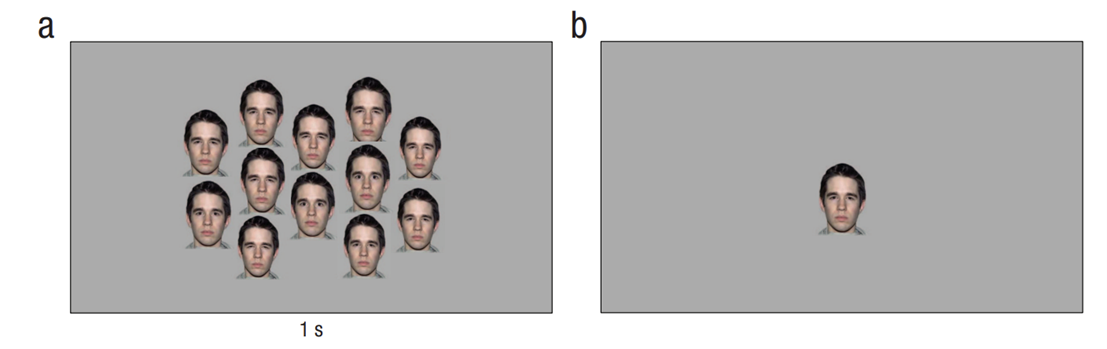
\includegraphics{D:/R/rdata/rbighomework/Re_Goldenberg_2021_Group2_2023/picture/Faces_material1.png}
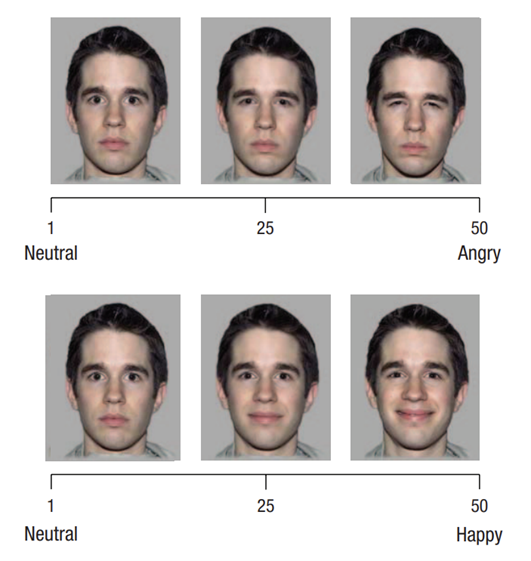
\includegraphics{D:/R/rdata/rbighomework/Re_Goldenberg_2021_Group2_2023/picture/Faces_material2.png}
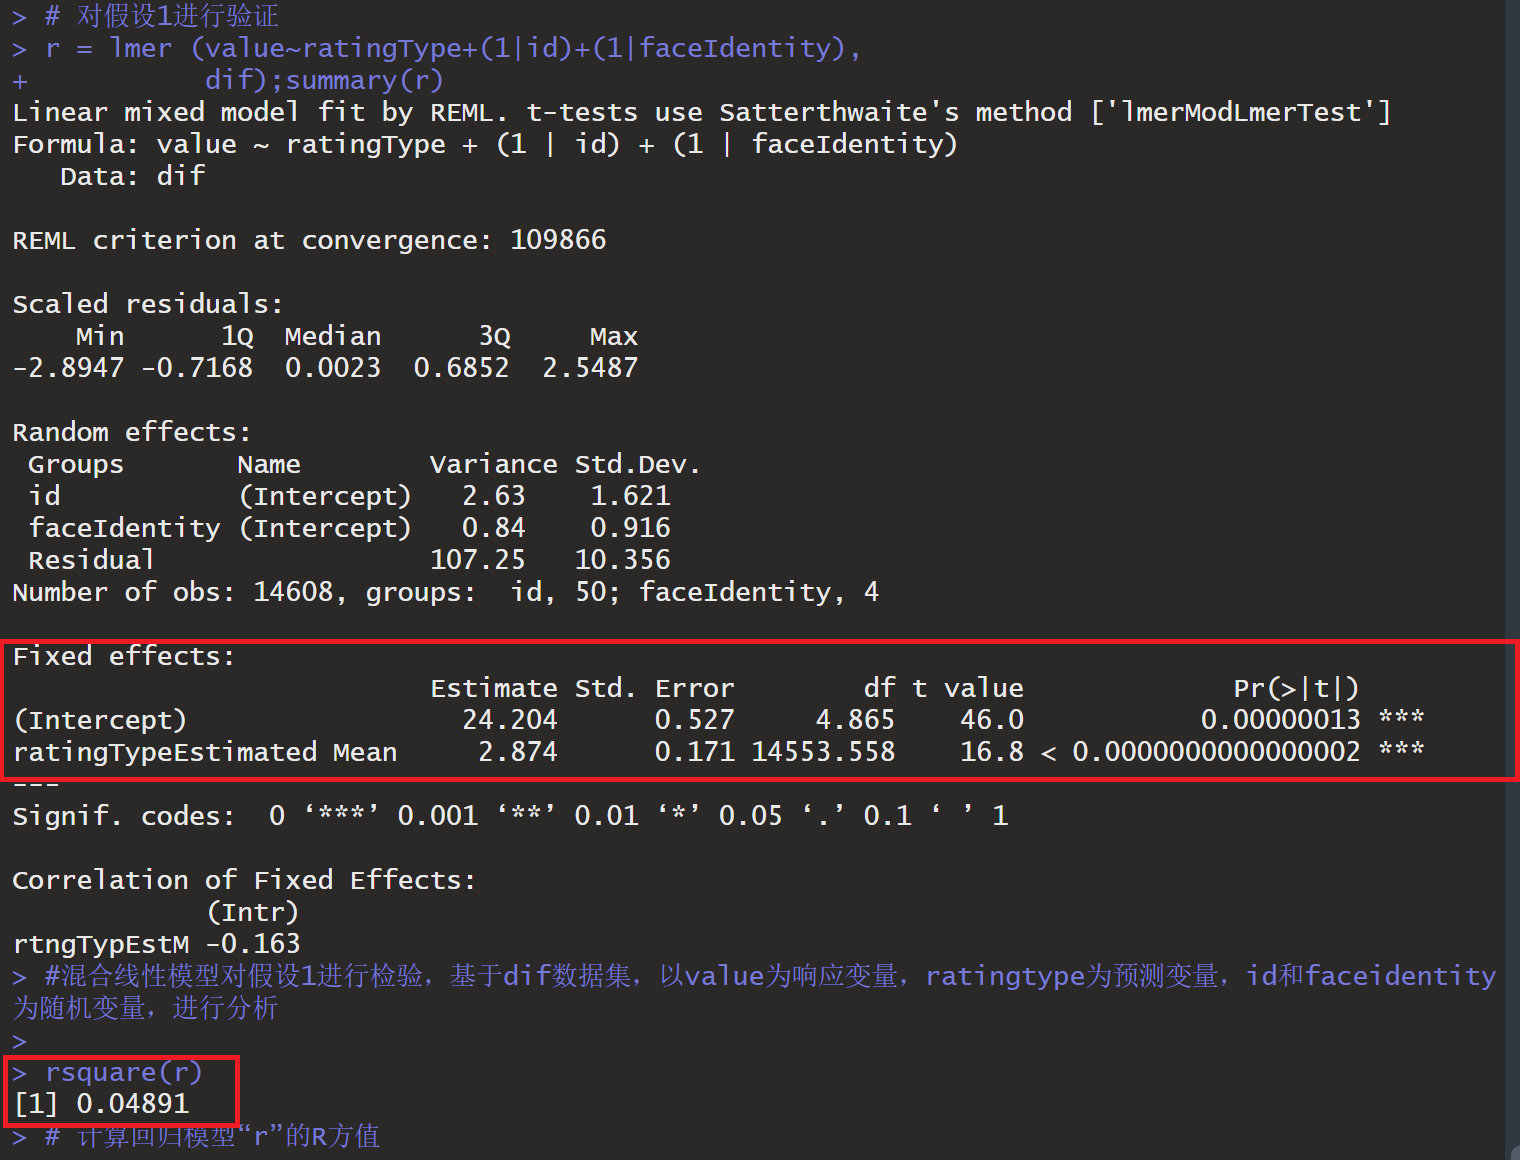
\includegraphics{D:/R/rdata/rbighomework/Re_Goldenberg_2021_Group2_2023/picture/mix_model.png}
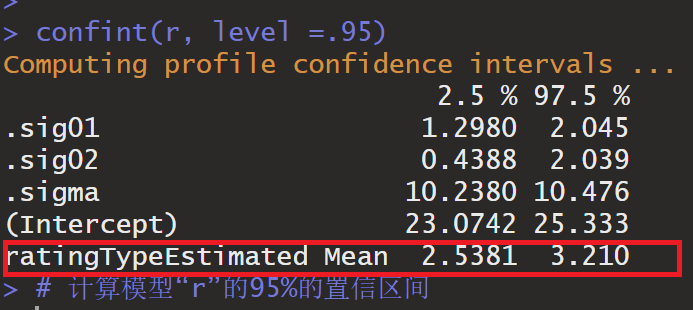
\includegraphics{D:/R/rdata/rbighomework/Re_Goldenberg_2021_Group2_2023/picture/confidence_intervals.png}
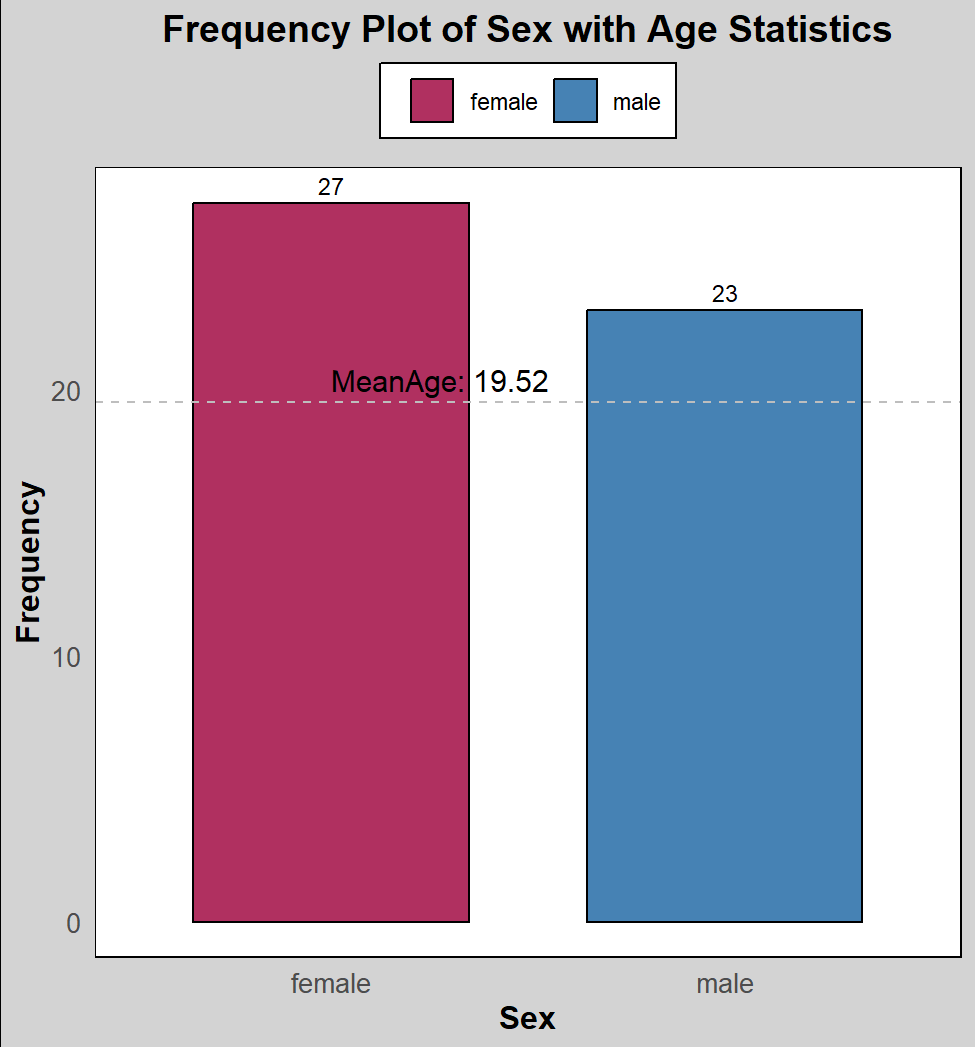
\includegraphics{D:/R/rdata/rbighomework/Re_Goldenberg_2021_Group2_2023/picture/descript.png}
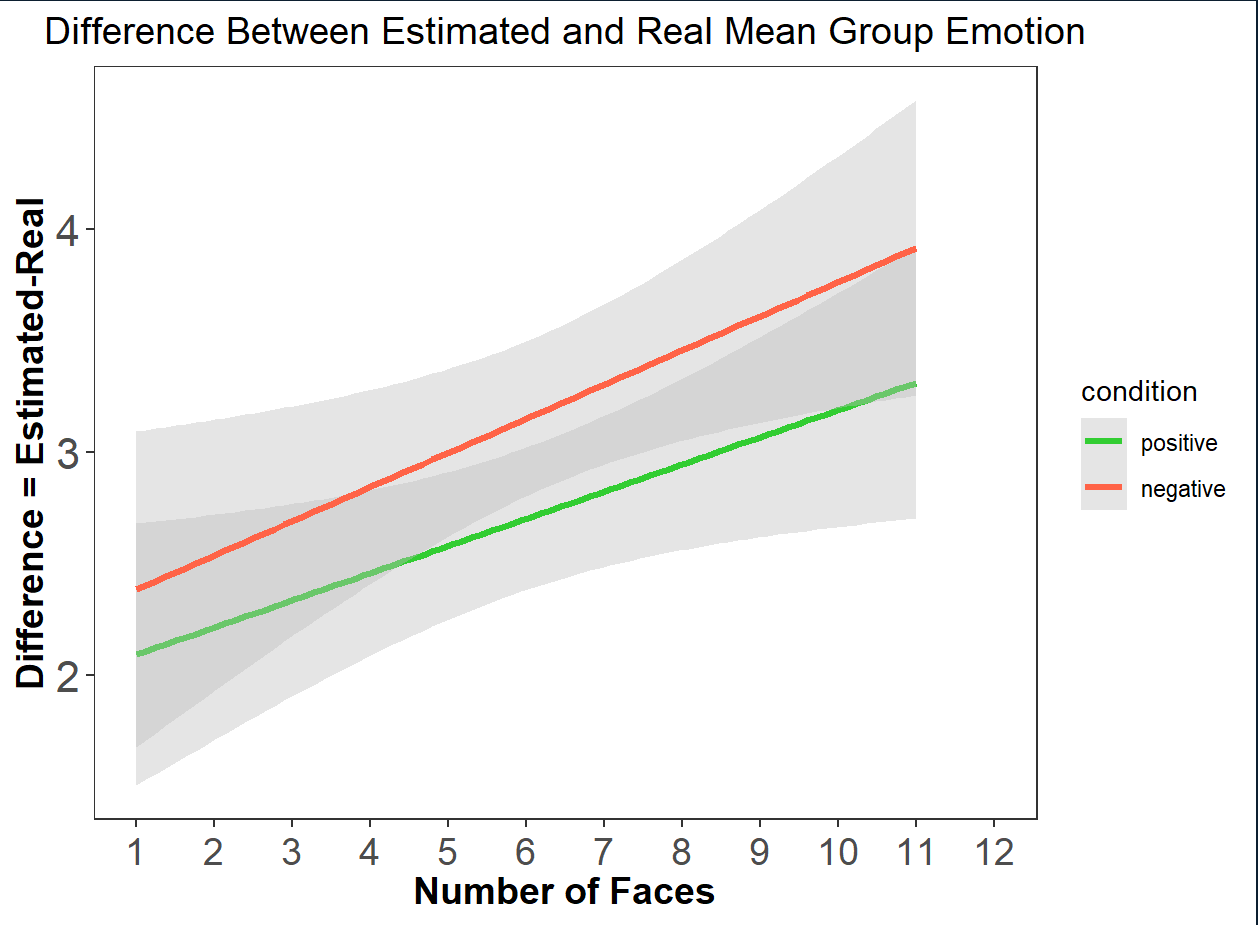
\includegraphics{D:/R/rdata/rbighomework/Re_Goldenberg_2021_Group2_2023/picture/hypothesis.png}
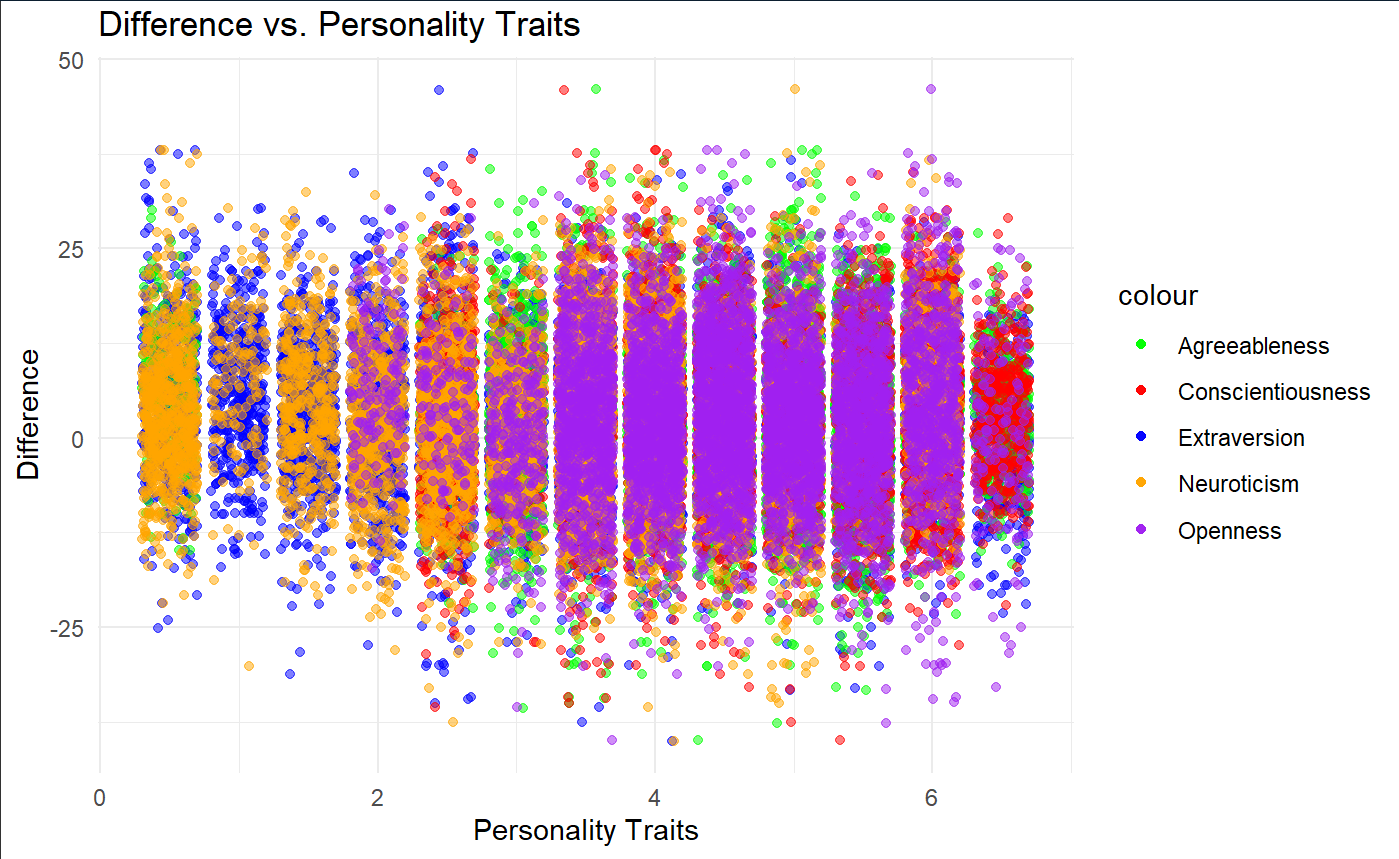
\includegraphics{D:/R/rdata/rbighomework/Re_Goldenberg_2021_Group2_2023/picture/Exploratory.png}


\end{document}
